\documentclass{article}
\usepackage{float}
\usepackage{graphicx} % Required for inserting images

\title{Assignment 4 : String Search}
\author{Kanishka Jayathilake}
\date{February 2025}

\begin{document}

\maketitle

\section{Introduction}

The main purpose of this experiment is to compare the performance of Naive and Boyer Moore Search across different text sizes. Both algorithms are used for pattern matching, but their approaches differ significantly. Naive Search follows a brute-force approach, checking every possible position in the text where the pattern might appear. It can be slow for large text sizes. Boyer-Moore Search optimizes the process by skipping unnecessary comparisons using the bad character rule and good suffix rule, making it more efficient in most cases.

This experiment focuses on runtime performance and memory usage for both algorithms. By analyzing how their performance changes with increasing text sizes, our goal is to determine whether Boyer-Moore consistently outperforms Naive Search and in what cases Naive Search might still be useful.

\section{Result}

This experiment generated two key graphs, one for runtime analysis and another for memory usage.

In the runtime analysis graph, Boyer-Moore demonstrated consistently better performance, with runtime remaining stable even as text size increased. Naive Search. However that graph  showed large fluctuations with major spikes at text sizes around 1250 and 1750 characters. These spikes suggest that the efficiency of Naive Search is highly dependent on the text’s structure and how often the pattern appears. 

The memory usage graph showed that Naive Search consistently used more memory than Boyer-Moore. The memory consumption for Naive Search was around 150 or more bytes, while Boyer-Moore remained closer to 100 bytes. This suggests that Boyer-Moore is not only faster but also more memory-efficient, making it the better choice for large-scale searches. While both algorithms required more memory as the text size increased, Boyer-Moore maintained a lower and more stable memory usage than Naive search.



\begin{figure}[H] 
    \centering
    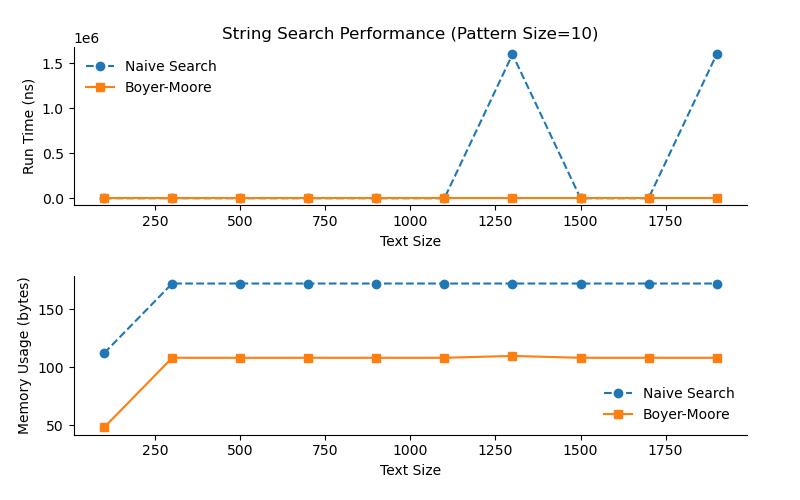
\includegraphics[width=0.7\textwidth]{results.png}
    \caption{Result Graphs}
    \label{fig:results}
\end{figure}



\section{Method}

For this experiment, a series of random text strings and patterns were generated to test each algorithm under controlled conditions. The text sizes ranged from 100 to 2000 characters, increasing in steps of 200 characters. The patterns used for searching were randomly generated with a fixed length of 10 characters.

To ensure accuracy, each search algorithm was tested 10 times per text size, and the average runtime and memory usage were recorded. Runtime was measured in nanoseconds to track execution speed, while memory usage was measured in bytes. The same randomly generated texts and patterns were used for each test, ensuring fair comparisons between Naive Search and Boyer Moore.

One important factor considered was how the distribution of characters in the text affects performance. Since Boyer Moore relies on skipping sections of text, its efficiency improves when the text contains diverse characters that trigger more skips. Naive Search doesn't benefit from such variations and performs similarly regardless of character distribution.

\subsection{Reproducibility}

 To replicate these experiments, clone the repository and then run the empirical and simulation experiments as
 follows:

 \begin{enumerate}
    \item \textbf{Clone the repository} using the following command:
    \begin{verbatim}
    git clone https://github.com/cu-compg-spring-2025/assignment-4-searching-KMJayathilake.git
    \end{verbatim}

    \item \textbf{Navigate to the source directory}:
    \begin{verbatim}
    cd src
    \end{verbatim}

    \item \textbf{Run the experiment} with the specified parameters:
    \begin{verbatim}
    python string_search.py --text_range 100 2000 200 --pattern_size 10 --rounds 10 --out_file results.png

    \end{verbatim}
\end{enumerate}

 
 \section{Conclusion}

 From this experiment, it is clear that Boyer-Moore significantly outperforms Naive Search in most cases, particularly for larger text sizes. Naive Search becomes inefficient as text size increases, leading to noticeable spikes in runtime. However, for small text sizes  or when the pattern is very short, Naive Search still performs reasonably well.



\section{Appendix}

\item Used ChatGPT to edit and correct the grammar.
\item Used GitHub Copilot.

\end{document}

